\chapter{Probability space intro}
\section{probability space}
我们这里跳过所有 measure theory 的内容, 见 notes on measure theory.\\
\begin{definition}{prob space, prob measure, sample space, event space}
    一个 probability space 就是一个 measure space \( (\Omega, \mathcal{F}, \mathbb{P}) \), 其中 $\mathbb{P}(\emptyset) =0, \mathbb{P}(\Omega) = 1$.\\
    对于这样的 measure $\mathbb{P}$, 我们称之为 \textbf{probability measure (概率测度, 即概率)}.\\
    而这里的 \(\Omega\) 我们称之为 \textbf{sample space (样本空间)}; 这里的 $\sigma$-algebra $\mathcal{F}$, 我们称之为 \textbf{event space (事件空间)}. \\
    任意的 $A \subset \Omega$ 都是一个 \textbf{event}, 但是概率论中只考虑 $A\in\mathcal{F}$, 即 measurable event. 为简化, event 这个单词就指 measurable event.
\end{definition}
\begin{remark}
    回顾一下 measure space 的定义:
    \begin{itemize}
        \item 一个 set $\Omega$ 的一个 $\sigma$-algebra 就是一个包含空集的子集簇, 其 \textbf{closed under countable unions and complements}. (如果只 closed under finite unions, 则只称为一个 algebra.)
        \item 一个 Borel algebra 是一个定义在 topological space 上的 $\sigma$-algebra, 由 all open sets 生成. (因而: closed under countable unions and complements.) $\mathbb{R}$ 的 Borel algebra 可以由 all open intervals 生成.
        \item 一个 measure on a measurable space $(\Omega, \mathcal{F})$ 就是一个从 $\mathcal{F} \to \mathbb{R}$ 的函数, 满足 \textbf{countable additivity}.
        \item measure 的性质: \textbf{(1)non-negativity, (2) monotonicity, (3) countable subadditivity, (4) inclusion-exclusion principle (上节已讲), (5) continuity from below and above.} 第 (5) 条具体即:
        For measurable sets $A_1 \subseteq A_2 \subseteq \cdots \subseteq A_n \subseteq \cdots$, then $\lim_{n \to \infty} \mathbb{P}(A_n) = \mathbb{P}(\bigcup_{n=1}^{\infty} A_n)$.\\
        For measurable sets $A_1 \supseteq A_2 \supseteq \cdots \supseteq A_n \supseteq \cdots$, then $\lim_{n \to \infty} \mathbb{P}(A_n) = \mathbb{P}(\bigcap_{n=1}^{\infty} A_n)$.
    \end{itemize}
\end{remark}
\begin{remark}
    对于 discrete 的 prob space 而言, 通常选取 $\mathcal{F} = 2^{\Omega}$, 即 $\Omega$ 的任意子集都是一个 event.
\end{remark}
\begin{remark}
    概率空间的现实意义是: 一次 experiment 的所有可能的结果的集合, 以及每个结果的概率.
    \begin{align*}
        \Omega &= \{\omega \mid \omega \text{ 是一次 experiment 的可能的结果}\}\\
        \mathbb{P}(\omega) &= \text{ 结果 $\omega$ 的可能性}
    \end{align*}
\end{remark}

\begin{example}
    (dice roll) 
    如果我们掷一个 6 面的骰子, 那么样本空间 $\Omega=\{1,2,3,4,5,6\}$. 一个可能的事件是 $A=\{1,2\}$. 如果假设骰子是公平的 (所有结果都是等可能的), 那么事件 $A$ 的概率是
    \[
    \mathbb{P}(A)=\frac{\text { Number of favorable outcomes }}{\text { Total number of outcomes }}=\frac{|A|}{|\Omega|}=\frac{2}{6} 
    \]
    % 如果我们定义一个随机变量 $X$ 表示掷骰子的结果, 那么 $X$ 的样本空间是 $\mathbb{R}$, 即 $X: \Omega \rightarrow \mathbb{R}$. 
    % 那么 $X$ 的分布函数是
    % \[
    % F_X(x) = \mathbb{P}(X \leq x) = \begin{cases}
    %     0, & x < 1 \\
    %     1/6, & 1 \leq x < 2 \\
    %     2/6, & 2 \leq x < 3 \\
    % \end{cases}
    % \]
    根据我们 measure-based 的定义, 这一结果自然 follows from countable additivity of $\mathbb{P}$.
\end{example}




\begin{example}
    三个人独立地掷一个 6 面的骰子, 求第三个人掷出的点数等于前两个人的点数之和的概率.
    \begin{solution}
        样本空间 $\Omega=\{1,2,3,4,5,6\}^3$.
        event: $E = \{ \omega \in \Omega \mid \omega_3 = \omega_1 + \omega_2 \}$.\\
        这个 event 有 15 个 elements: \[
        E = \{ (1,1,2), (1,2,3), (1,3,4), \cdots, (2,1,3), (2,2,4), \cdots, (3,1,4), \cdots, (4,1,5), \cdots, (5,1,6) \}
        \]
        因此, 概率是: \[
        \mathbb{P}(A)=\frac{|A|}{|\Omega|}=\frac{15}{216}=\frac{5}{72}
        \]
    \end{solution}
\end{example}


\begin{example}
    两个人计划在 12:00 到 1:00 之间碰面. 他们各自都会在期间的某个时间点到达. 求: 他们彼此不会等待对方超过 10 分钟的概率.\\
    \begin{solution}
        Sample space $$\Omega = \{(x,y): 0\leq x \leq 60, 0\leq y \leq 60\} = [0,60] \times [0,60]$$
        我们要求概率的事件 \[
        E = \{ (x,y)\in \Omega : |x-y| \leq 10 \} 
        \]
        容易画出图像:
        \begin{center}
        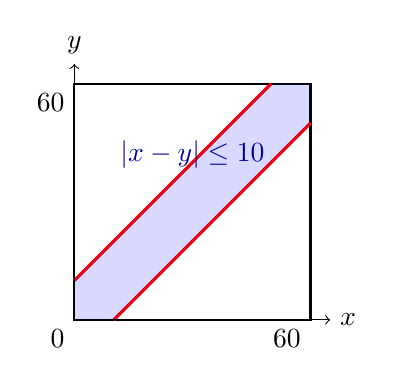
\begin{tikzpicture}[scale=0.05]
            % 绘制正方形区域
            \draw[thick] (0,0) rectangle (60,60);
            % 绘制两条界限直线: x-y=10  与 x-y=-10
            \draw[red,very thick] (10,0) -- (60,50);   % x - y = 10
            \draw[red,very thick] (0,10) -- (50,60);   % x - y = -10
            % 填充有效区域
            \fill[blue,opacity=0.15] 
                (0,10) -- (10,0) -- (60,50) -- (50,60) -- cycle;
            % 漏画了两个小的角
            \fill[blue,opacity=0.15]
                (0,0) -- (0,10) -- (10,0) -- cycle;
            \fill[blue,opacity=0.15]
                (60,60) -- (60,50) -- (50,60) -- cycle;
            % 坐标轴
            \draw[->] (0,0) -- (65,0) node[right] {$x$};
            \draw[->] (0,0) -- (0,65) node[above] {$y$};
            % 标注几个重要点
            \foreach \p/\lab in {(0,0)/0, (60,0)/60, (0,60)/60} {
                \draw \p node[below left]{\lab};
            }
            % 标签
            \node[blue!60!black] at (30,42) {$|x-y|\leq 10$};
        \end{tikzpicture}
        \end{center}
        因而概率是
        \[
        \mathbb{P}(E) = \frac{m(E)}{m(\Omega)} = \frac{3600-2500}{3600} = \frac{11}{36}
        \]
    \end{solution}
\end{example}



\section{conditional probability and independence}
\begin{definition}{conditional probability}
    对于 probability space \((\Omega, \mathcal{F}, \mathbb{P})\), 给定一个 event $B \in \mathcal{F}$, 我们定义 conditional probability of an event $A \in \mathcal{F}$ given $B$ 为:
    \[
    \mathbb{P}(A \mid B) = \frac{\mathbb{P}(A \cap B)}{\mathbb{P}(B)}
    \]
\end{definition}
\begin{proposition}{decomposing probability of intersection of events}   
    令 $\left(A_i\right)_{i \in \mathbb{N}}$ 为一个 seq of events, 对于任意 $n \in \mathbb{N}$:
    \[
    \mathbb{P}\left(A_1 \cap A_2 \cap \ldots \cap A_n\right)=\mathbb{P}\left(A_1\right) \cdot \mathbb{P}\left(A_2 \mid A_1\right) \cdot \mathbb{P}\left(A_3 \mid A_1 \cap A_2\right) \ldots \cdot \mathbb{P}\left(A_n \mid A_1 \cap \ldots \cap A_{n-1}\right)
    \]
\end{proposition}
\begin{proof}
Naturally follows from the def. 
\end{proof}


\begin{theorem}{law of total probability}
    令 $\left(A_i\right)_{i \in \mathbb{N}}$ 为一个 seq of \textbf{pairwise disjoint} events, 如果 $\sqcup_{i=1}^{\infty} A_i=\Omega$, 那么对于任意 event $E \subseteq \Omega$:
    \[
    \mathbb{P}(E)=\sum_{i=1}^{\infty} \mathbb{P}\left(A_i\right) \mathbb{P}\left(E \mid A_i\right)
    \]
\end{theorem}
\begin{proof}
    \[
    \mathbb{P}(E)=\mathbb{P}\left(E \cap \cup_{i=1}^{\infty} A_i\right)=\mathbb{P}\left(\cup_{i=1}^{\infty} E \cap A_i\right)=\sum_{i=1}^{\infty} \mathbb{P}\left(E \cap A_i\right)=\sum_{i=1}^{\infty} \mathbb{P}\left(A_i\right) \mathbb{P}\left(E \mid A_i\right)
    \]
\end{proof}
\begin{remark}
    \(P(A_i)P(E\mid A_i)\) 就等于 \(P(E \cap A_i)\), 也就是在 \(A_i\) 这个区域上, \(E\) 的 measure. 因而 disjoint union 之下就是 \(E\) 的完整 measure.
\end{remark}

\begin{theorem}{Bayes theorem}
    If $A, B \subseteq \Omega$ such that $\mathbb{P}(B) \neq 0$, then
    \[
    \mathbb{P}(A \mid B)=\frac{\mathbb{P}(A) \cdot \mathbb{P}(B \mid A)}{\mathbb{P}(B)}
    \]
\end{theorem}
\begin{remark}
    这其实是一个非常直接的结果, 因为 \(P(A) \dot P(B \mid A) = P(A \cap B)\). \\
    但是它的意义在于, 如果我们知道两个事件的概率和其中一个对另一个的条件概率, 我们就也得到了反过来的条件概率.
\end{remark}



\begin{example}{(Medical testing)}

在一个群体中, 随机选取一个人患有某种罕见疾病的概率是 0.001. 该疾病有一个诊断测试, 其性质如下: 给定个体患病, 测试呈阳性的概率 (真正阳性率) 是 0.99. 给定个体健康, 测试呈阳性的概率 (假阳性率) 是 0.02. 从群体中随机选取的一个人测试呈阳性. 该个体实际上患有该疾病的概率是多少?
于是
\begin{solution}
由 law of total probability, 我们有
\[
 \mathbb{P}(\text {positive})= \mathbb{P}(\text{positive} \mid \text{sick}) \mathbb{P}(\text{sick}) + \mathbb{P}(\text{positive} \mid \text{healthy}) \mathbb{P}(\text{healthy}) = 0.99 \cdot 0.001 + 0.02 \cdot 0.999 = 0.02097
\]
于是
\[
\mathbb{P}(\text {sick} \mid \text {positive})=\frac{0.99 \cdot 0.001}{0.02097} \approx 0.047
\]
\end{solution}
\end{example}

\begin{example}{(Monty Hall problem)}
假设你参加一个游戏节目, 面前有三扇门: 一扇门后面有一辆车; 其他两扇门后面是山羊. 你选择了一扇门, 比如说是 1 号门, 然后主持人 (他知道每扇门后面是什么) 打开了另一扇门, 比如说是 3 号门, 里面有一只山羊. 然后他说 "你想换成 2 号门吗?". 换门对你有利吗?
\begin{solution}
令 \(A_i\) 表示: car 在 \(i\) 号门后面; \(B\) 事件表示: 主持人打开 3 号门. 我们要求的概率是在事件 \(B\) 发生的情况下, \(A_2\) 的个概率, 即 \(\mathbb{P}(A_2 \mid B)\). 它的大小是:
\begin{align*}
\mathbb{P}(A_2 \mid B) &= \frac{\mathbb{P}(A_2) \cdot \mathbb{P}(B \mid A_2)}{\mathbb{P}(B)} \\
&= \frac{\mathbb{P}(B \mid A_2)\mathbb{P}(A_2)}{\mathbb{P}(B\mid A_1)\mathbb{P}(A_1) + \mathbb{P}(B\mid A_2)\mathbb{P}(A_2) + \mathbb{P}(B\mid A_3)\mathbb{P}(A_3)}    \\
&= \frac{1 \cdot \frac{1}{3}}{\frac{1}{2} \cdot \frac{1}{3} + 1 \cdot \frac{1}{3} + 0 \cdot \frac{1}{3}} = \frac{2}{3} > \frac{1}{3}
\end{align*}
因而, 换门是有利的.
\end{solution}
\end{example}